\documentclass[11pt,a4paper]{article}

\usepackage[T1]{fontenc}
\usepackage[utf8]{inputenc}
\usepackage{lmodern}
\usepackage{microtype}
\usepackage[margin=2.5cm]{geometry}
\usepackage{amsmath}
\usepackage{booktabs}
\usepackage{tabularx}
\usepackage{siunitx}
\usepackage{enumitem}
\usepackage{tikz}
\usetikzlibrary{positioning,arrows.meta}
\usepackage[numbers,sort&compress]{natbib}
\usepackage[hidelinks]{hyperref}
\usepackage{xurl}

\sisetup{group-separator={,},group-minimum-digits=4}
\setlist{itemsep=2pt,topsep=4pt}

\title{Superblocks for Budapest:\\automated design, impact assessment\\and an implementation pathway}
\author{Gergely Varhelyi-Toth}
\date{November 2026}

\begin{document}
\maketitle

\begin{abstract}
\noindent A superblock is a group of city blocks, typically 6 to 20\,ha, whose interior streets are closed to through motor traffic while every address keeps car access. Through traffic is kept on a surrounding grid of main roads, and the freed interior street space can be given to walking, cycling, play and greenery.
We present Superblocker, an open-source tool that designs a superblock plan for a whole city automatically from OpenStreetMap, and apply it to Budapest. The tool chooses the boundary-road network, divides the city into cells, places modal filters, one-way changes, bus gates and camera-enforced destination-only gates, and verifies on the routing graph that no car can cross a cell between two main roads while every junction stays reachable. It then tests the plan in a city-wide traffic, NO$_2$ and noise model built only from open data.
For Budapest the tool produces 2,598 cells in about 100\,s. All cells pass the through-traffic test, none of the roughly 4,200 main-road entries can reach another main road through residential streets, and no junction loses car access; the plan needs about 1,300 destination-only gates.
The impact model is less favourable. With a modest trip response (elasticity $-0.5$), average peak car trips take about 21\% longer, network capacity falls by about 19\%, and population-weighted NO$_2$ rises slightly (22.4 to 22.8\,\si{\micro\gram\per\cubic\metre}), because diverted traffic concentrates on main roads lined with homes. An 800\,HUF entry charge at the Hungária ring calms the centre but moves cross-river traffic to the free ring.
We conclude that a city-wide superblock grid is technically constructible for Budapest, but should be built district by district from trial installations, together with measures that reduce car demand, and with measured traffic counts before any number here is quoted as a forecast.
\end{abstract}

\section{Introduction}

Most residential streets in a European city carry traffic that has neither its origin nor its destination there. Navigation apps route drivers onto any street that saves a minute, so quiet streets become rat runs, bringing noise, NO$_2$, crash risk and a carriageway children cannot use.

The superblock (Catalan \emph{superilla}) answers this with network design rather than with speed humps. A cluster of blocks is ringed by main roads that carry through traffic. Inside, a few modal filters, one-way loops or gates make every route between two main roads longer than the route around, while residents, deliveries and emergency services still reach every door. The concept was developed by Salvador Rueda and the Barcelona Urban Ecology Agency \citep{rueda2019}; Barcelona's 2016 programme, Ghent's 2017 circulation plan and London's low-traffic neighbourhoods are its best documented applications.

Designing such a plan by hand is slow and error-prone. A filter in the wrong place strands a street, sends traffic through the next block, or blocks a bus route. Most cities therefore build one superblock at a time, and nobody checks what the whole grid would do. This paper asks three questions for Budapest:
\begin{enumerate}
  \item Can a complete superblock plan for the whole city be generated automatically from open data, and verified to remove through traffic without cutting off any address?
  \item What would such a plan do to car travel times, network capacity, air quality and noise, city-wide and for the people who live on the main roads?
  \item What would it take to build it in Budapest: in law, in money, in sequence and in evidence?
\end{enumerate}
Our contributions are an open-source design algorithm with formal validity checks (Section~\ref{sec:method}), a city-wide screening model using only open data (Sections~\ref{sec:data} and~\ref{sec:method}), results for Budapest with their uncertainties stated (Sections~\ref{sec:results} and~\ref{sec:limits}), and an implementation pathway grounded in what worked and failed elsewhere (Section~\ref{sec:implementation}).

\section{Background and related work}

The evidence on superblocks and their relatives is consistent on the inside of a scheme and contested on its edge: inside, traffic falls a lot; on the boundary, outcomes depend on how much traffic disappears rather than diverts.

\paragraph{Barcelona.} The Poblenou and Sant Antoni superblocks cut interior traffic sharply; Sant Antoni saw NO$_2$ fall about 25\% and noise about 3.5\,dB. A health impact assessment of the full 503-superblock vision estimated about 667 premature deaths avoided each year, mainly from less NO$_2$, noise and heat and more physical activity \citep{mueller2020}. That estimate assumes much of the displaced traffic disappears.

\paragraph{Ghent.} In 2017 Ghent divided its centre into six sectors that cars can only move between via the ring. Peak car traffic fell about 12\%, cycling rose about 25\% and public transport about 28\%. Ghent is the closest precedent to a whole-city design.

\paragraph{London low-traffic neighbourhoods.} Inside London's LTNs motor traffic fell about 48\%, while boundary roads changed only marginally on average \citep{thomas2024}. Results vary widely between schemes, and boundary-road congestion is the most common public objection.

\paragraph{Traffic evaporation.} A review of about 100 road-space reductions found traffic on the treated roads fell 41\% on average, and less than half of it reappeared on nearby roads \citep{cairns2002}. Evaporation is real but not guaranteed; it depends on alternatives existing.

\paragraph{Road pricing.} Stockholm's cordon cut entries by 20--22\% and held at 18--20\%; Milan's Area~C by 30--38\%; London's area charge by 18\%; Gothenburg's by 12\%, with its bypasses 16--26\% busier \citep{eliasson2009,borjesson2015,cts2012,itf,danielis}. Pricing reduces demand, whereas filters only redistribute it. London's experience is that taking road space away without pricing lets congestion return while volumes stay down.

\paragraph{Automated design.} \citet{eggimann2022} identified candidate superblocks in many cities from street-network geometry, showing the potential is large and widespread. To our knowledge no published tool designs the filter placement for a whole city, verifies the result free of through routes and stranded addresses, and tests it in a city-wide traffic assignment. That is the gap this paper addresses.

\paragraph{Budapest.} Budapest has district-level traffic calming and some \emph{kivéve célforgalom} (access only) streets, but no superblock programme. An inner-city entry charge has been studied since 2008 \citep{origo2013} and is in the 2019 Mobility Plan \citep{bkk}, but Hungarian road law does not let the capital levy it \citep{kuria2024} (Section~\ref{sec:implementation}).

\section{Data}\label{sec:data}

Every input is open and needs no account, so the study can be repeated by anyone and for any city (Table~\ref{tab:data}). The one input Budapest does not publish openly, traffic counts, is the study's largest weakness.

\begin{table}[ht]
\centering\small
\caption{Data layers.}\label{tab:data}
\begin{tabularx}{\linewidth}{@{}>{\raggedright}p{3.2cm}>{\raggedright}X>{\raggedright}p{1.5cm}>{\raggedright\arraybackslash}X@{}}
\toprule
Layer & Source & Licence & Use \\
\midrule
Street network (34,641 junctions) & OpenStreetMap via OSMnx \citep{boeing2017}, inside the Nominatim boundary & ODbL & Cells, filters, routing, capacities \\
Turn restrictions & OSM relations via Overture Maps & ODbL & Movement-level routing \\
Bus, trolleybus, tram routes & OSM; BKK GTFS feed & ODbL; BKK & Bus gates; walking access to stops \\
Fire, ambulance, schools & OSM; Overture places & ODbL; CDLA & Emergency response; school streets \\
Residents & Meta High Resolution Settlement Layer, 30\,m & CC BY 4.0 & Trip origins; exposure weighting \\
Jobs (proxy) & Overture places and buildings & CDLA, ODbL & Trip destinations \\
NO$_2$ annual means 2025 & 10 Budapest stations via OpenAQ & CC BY 4.0 & Fitting the NO$_2$ model \\
Entry-charge cordon & Hungária ring and Buda inner ring (32\,km$^2$) & ODbL & Entry charge scenario \\
Traffic counts & None openly available & -- & Would calibrate demand and boundary roads \\
\bottomrule
\end{tabularx}
\end{table}

The software is written in Python 3.12 (FastAPI, OSMnx, NetworkX, GeoPandas, Shapely) with a React, MapLibre and deck.gl interface, and is released under GPL-3.0 at \url{https://github.com/tgergo1/Superblocker}.

\section{Method}\label{sec:method}

The method has two halves (Figure~\ref{fig:pipeline}). The design half builds a plan and verifies two properties on the routing graph: no through route, and no address cut off. The assessment half asks what the plan does to the city in a traffic, air and noise model.

\begin{figure}[ht]
\centering
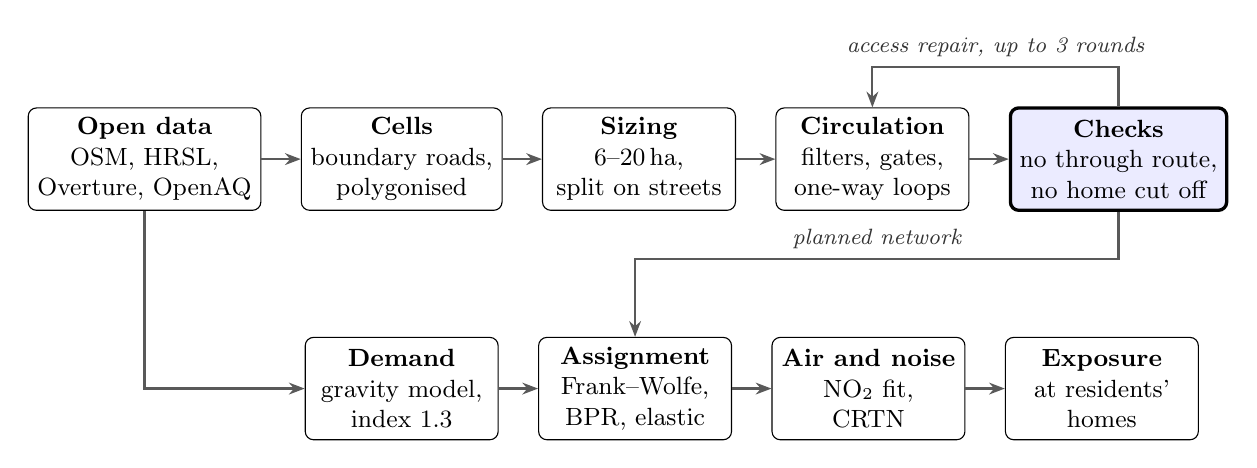
\begin{tikzpicture}[
  node distance=5mm and 5mm,
  box/.style={draw, rounded corners=3pt, align=center, minimum width=2.45cm, minimum height=1.3cm, font=\small},
  key/.style={box, very thick, fill=blue!8},
  arr/.style={-{Stealth[length=2mm]}, thick, gray!70!black},
  lab/.style={font=\footnotesize\itshape, gray!40!black}]
  \node[box] (data) {\textbf{Open data}\\OSM, HRSL,\\Overture, OpenAQ};
  \node[box, right=of data] (cells) {\textbf{Cells}\\boundary roads,\\polygonised};
  \node[box, right=of cells] (size) {\textbf{Sizing}\\6--20\,ha,\\split on streets};
  \node[box, right=of size] (circ) {\textbf{Circulation}\\filters, gates,\\one-way loops};
  \node[key, right=of circ] (check) {\textbf{Checks}\\no through route,\\no home cut off};
  \node[box, below=16mm of cells] (dem) {\textbf{Demand}\\gravity model,\\index 1.3};
  \node[box, right=of dem] (assign) {\textbf{Assignment}\\Frank--Wolfe,\\BPR, elastic};
  \node[box, right=of assign] (env) {\textbf{Air and noise}\\NO$_2$ fit,\\CRTN};
  \node[box, right=of env] (exp) {\textbf{Exposure}\\at residents'\\homes};
  \draw[arr] (data) -- (cells);
  \draw[arr] (cells) -- (size);
  \draw[arr] (size) -- (circ);
  \draw[arr] (circ) -- (check);
  \draw[arr] (check.north) -- ++(0,5mm) -| node[lab, pos=0.25, above] {access repair, up to 3 rounds} (circ.north);
  \draw[arr] (data.south) |- (dem.west);
  \draw[arr] (check.south) -- ++(0,-6mm) -| node[lab, pos=0.25, above] {planned network} (assign.north);
  \draw[arr] (dem) -- (assign);
  \draw[arr] (assign) -- (env);
  \draw[arr] (env) -- (exp);
\end{tikzpicture}
\caption{Design and assessment pipeline. The top row designs the plan and loops through the access repair until every check passes; only a valid plan enters the city-wide traffic, air and noise model in the bottom row.}\label{fig:pipeline}
\end{figure}

\subsection{Boundary roads and cells}
The street graph is loaded inside the city's administrative polygon. Boundary roads are chosen from measured counts when they exist; otherwise from road class (motorway to secondary, plus busy tertiary roads) and sampled betweenness centrality. The boundary network is polygonised into closed cells and clipped to the city boundary. Motorways and trunk roads are corridors the plan never modifies.

\subsection{Sizing}
Cells are merged and split towards a target of 12\,ha, with 6\,ha and 20\,ha as the limits. An oversized cell is split along the whole length of a residential street, followed through its junctions to the boundary roads. Among candidate splits, the one chosen divides the area most evenly while keeping its least compact piece compact, measured by the Polsby--Popper score \citep{polsby1991}
\begin{equation}
  PP = \frac{4\pi A}{P^{2}},
\end{equation}
where $A$ is the piece's area and $P$ its perimeter. A split street gets a filter halfway along so that it does not become a new rat run. Housing estates served only by living streets may split along them as a last resort. Three kinds of cell are reported separately rather than forced into range: cells already calm (all interior streets are dead ends from one entry), cells that are mostly open land, and undividable blocks where every split leaves a sliver.

\subsection{Circulation design}
Every junction where a cell's streets meet a boundary road is an entry. Entries are grouped into sectors (four by default, falling back to three and then two when a design cannot keep access). A constraint solver chooses the cheapest set of changes so that no directed path inside the cell links two different sectors; the changes, in rising cost, are a one-way conversion, a modal filter and a full street cut. A filter on a bus, trolleybus or tram route becomes a camera bus gate; other filters are emergency bollards. Where every cut that would close a route also strands homes, the closure becomes a camera-enforced destination-only gate that residents, deliveries and visitors may pass.

\subsection{Validity checks}
A plan is accepted only when it passes three checks on the routing graph. Through traffic is routed as an ordinary car; access is routed as a resident who may pass destination-only gates.
\begin{enumerate}
  \item \textbf{No through route.} For each cell, no car path enters at one sector and leaves at another.
  \item \textbf{No crossing.} No car entering from a main road can reach another main-road junction through residential streets, including across neighbouring cells. A seal pass adds filters (up to 30 per entry) until this holds.
  \item \textbf{No stranded junction.} On the whole planned city, every junction reachable by car today stays reachable in and out. An access repair reopens the cheapest change for each stranded pocket (a one-way first, then a split-street filter, then an interior filter), turns it into a gate when reopening would recreate a through route, and redesigns the affected cells for up to three rounds.
\end{enumerate}

\subsection{Traffic model}
The city is divided into 800\,m zones. Peak-hour car trips run between zones by a gravity model, from residents to jobs, with 15\% of trips entering or leaving through main-road gateways at the city edge. Demand is scaled so that today's average trip takes 1.3 times its free-flow time. Trips are assigned to user equilibrium by the Frank--Wolfe algorithm \citep{frank1956}, movement by movement (turn restrictions, junction delays by control type, U-turns only at dead ends), with BPR link costs \citep{bpr1964}
\begin{equation}
  t(v) = t_0\left[1 + 0.15\left(\frac{v}{c}\right)^{4}\right].
\end{equation}
Demand then responds to the plan with an elasticity of $-0.5$ on trip time, iterated with the assignment. Capacity is the demand multiple at which the average trip takes twice its free-flow time.

\subsection{Air and noise}
Each link emits NO$_x$ in proportion to its volume and a speed-dependent fleet emission factor, with a heavy-vehicle share by road type. Emissions are spread on a metric grid by a near-road kernel (exponential, 30\,m) and an urban-scale kernel (4\,km). Annual mean NO$_2$ at the ten stations is fitted by non-negative least squares,
\begin{equation}
  \mathrm{NO_2} = b_0 + a\,E_{\text{near}} + b\,E_{\text{urban}},
\end{equation}
with the two decay lengths chosen by leave-one-out error. Noise is the CRTN peak-hour level at 10\,m from each link \citep{crtn1988}, spread by inverse square and summed by energy, without screening by buildings. Both are counted at residents' homes.

\subsection{Entry charge}
A charge at the Hungária-ring cordon enters route choice as time at a value of time of 3,000\,HUF/h, so through traffic can go round. A trip whose route still enters the zone keeps a share of its demand
\begin{equation}
  s = e + (1-e)\left(\frac{C+p}{C}\right)^{\varepsilon},
\end{equation}
where $C$ is the trip's generalised cost (time at 3,000\,HUF/h plus 60\,HUF/km), $p$ the charge (800\,HUF central), $e=0.2$ the exempt share and $\varepsilon=-0.7$ (range $-0.5$ to $-1.2$, from Stockholm and Gothenburg at introduction \citep{cts2012,itf}). Zone residents are exempt. Junctions within 60\,m of the cordon count as outside, so the ring and the end bridges are free.

\section{Results}\label{sec:results}

The tool can build a valid superblock plan for all of Budapest, but the plan on its own makes driving slower and does not improve air quality on average. Figures come from three runs of the software at successive versions (October 2026); each table names its run. Cell counts differ between runs because the impact runs use the population layer, which changes which cells count as superblocks.

\subsection{The plan}

Table~\ref{tab:plan} gives the whole-city plan at default settings without traffic counts.

\begin{table}[ht]
\centering\small
\caption{Whole-Budapest plan (12\,ha target, 6--20\,ha limits).}\label{tab:plan}
\begin{tabular}{@{}lr@{}}
\toprule
Result & Value \\
\midrule
Cells & 2,598 \\
Cells passing the through-route check & 2,598 (100\%) \\
Main-road entries reaching another main road via residential streets & 0 of $\approx$4,200 \\
Junctions cut off from car access & 0 \\
Destination-only camera gates & $\approx$1,308 \\
Undividable blocks over 20\,ha (median 24\,ha) & 43 \\
Cells over 20\,ha that are mostly open land (median 48\,ha) & 120 \\
Superblocks under 6\,ha & 5 \\
Eligible road coverage of the boundary network & 99.8\% \\
Run time & $\approx$100\,s \\
\bottomrule
\end{tabular}
\end{table}

The destination-only gates are the price of validity. About 930 of them sit on split streets the access repair had to reopen, 760 of those on a single block-long section with no other place for a filter. A plan with only physical filters would strand homes or leave through routes.

\subsection{Traffic, air and noise}

Table~\ref{tab:impact} gives impact model v2 (2,313 superblocks, 646 bus gates, no motorway changes, 238,000 morning-peak car trips).

\begin{table}[ht]
\centering\small
\caption{Traffic impact of the plan against today.}\label{tab:impact}
\begin{tabular}{@{}lrr@{}}
\toprule
Measure & Fixed demand & Trips respond ($\varepsilon=-0.5$) \\
\midrule
Average car trip time & +21.5\% & +20.6\% \\
Car-km & +9.7\% & +4.0\% \\
Peak car trips not made by car & 0 & 8.7\% \\
Network capacity & $-19$\% & $-19$\% \\
Junctions cut off once filtered sections close & 11 & 11 \\
\bottomrule
\end{tabular}
\end{table}

The NO$_2$ fit reproduces the ten stations with $R^2=0.59$ and a leave-one-out error of 5.0\,\si{\micro\gram\per\cubic\metre}. Population-weighted annual NO$_2$ goes from 22.4 to 22.8\,\si{\micro\gram\per\cubic\metre}: 169,000 residents get at least 1\,\si{\micro\gram\per\cubic\metre} less and 307,000 at least 1 more. For noise, 281,000 residents get homes at least 3\,dB quieter and 240,000 at least 3\,dB louder.

The distribution matters more than the averages. Interior streets get much quieter and cleaner, but Budapest's main roads are lined with flats, so the people who take the diverted traffic are many. Without demand falling, the plan moves exposure rather than reducing it.

\subsection{Entry charge}

Table~\ref{tab:charge} compares the plan, an 800\,HUF charge per entry at the Hungária-ring cordon (32\,km$^2$, 108 charged entry links) and both together (205,825 morning-peak car trips, 2,123 superblocks, elasticity $-0.7$ with the range in brackets).

\begin{table}[ht]
\centering\small
\caption{Entry charge scenarios against today, once trips respond.}\label{tab:charge}
\begin{tabular}{@{}lrrr@{}}
\toprule
Measure & Superblocks & Charge & Both \\
\midrule
Cars entering the zone (57,600/h today) & +11\% & $-76$\% ($-75$ to $-79$) & $-68$\% ($-66$ to $-71$) \\
Driving inside the zone & +9\% & $-44$\% & $-34$\% \\
Main roads within 400\,m outside the zone & +49\% & +80\% & +111\% \\
Average car trip time & +19.4\% & +7.9\% & +25.8\% \\
Main roads more than 10\% busier & 773\,km & 335\,km & 751\,km \\
Peak car trips not made & 8.1\% & 3.1\% & 11.9\% \\
Residents $\geq$1\,\si{\micro\gram\per\cubic\metre} more / less NO$_2$ & 342k / 36k & 61k / 64k & 230k / 63k \\
Residents $\geq$3\,dB louder / quieter & 211k / 308k & 83k / 113k & 222k / 354k \\
Revenue per year & -- & 18\,bn HUF & 25\,bn HUF \\
\bottomrule
\end{tabular}
\end{table}

The charge calms the centre and, with the plan, cuts the residents breathing worse air from 342,000 to 230,000. It does not relieve the main roads the plan loads (773\,km against 751\,km), because cross-river traffic leaves the central bridges for the free ring and end bridges; peak flow on the Rákóczi bridge rises from about 5,200 to 9,100 vehicles an hour with the charge alone. At 400\,HUF the charge alone still cuts entries by 59\%: most of the effect is rerouting, not trips given up.

\section{Limitations and validity}\label{sec:limits}

The design checks are verifications on a graph; the impact numbers are screening estimates. The two should not be read with the same confidence.

\paragraph{What is verified, and on what.} The no-through-route, no-crossing and no-stranded-junction properties hold on the OpenStreetMap graph as mapped. They say nothing about map errors (a missing alley, a wrong one-way tag), private access roads, or addresses not snapped to the graph. The tool accepts an authoritative address dataset and checks each target, but none was used here.

\paragraph{No traffic counts.} Budapest publishes no open link counts. Demand is a gravity model calibrated to a single travel-time index of 1.3, and boundary roads come from road class and centrality. The modelled Hungária körút peaks at about 3,000 vehicles an hour, probably below reality. Every traffic figure is therefore relative (plan against today in the same model), not a forecast.

\paragraph{Static, single-class assignment.} Every driver takes the cheapest route at one value of time. Real drivers differ, and many would pay a charge or accept a slower route. This is why the modelled entry cut of $-68$ to $-79$\% is far beyond the $-12$ to $-30$\% measured elsewhere, and should be read as an upper bound.

\paragraph{Evaporation is probably understated.} The trip response gives 8.7\% fewer peak car trips. Measured schemes saw larger falls on treated roads (41\% on average \citep{cairns2002}), helped by better transit and cycling, which the model does not add. The trip-time and NO$_2$ penalties are closer to a pessimistic case than a central one.

\paragraph{Air and noise.} The NO$_2$ fit explains 59\% of the variance at only ten stations, treats chemistry as linear and uses a fleet-average emission factor. Noise ignores screening by buildings, so back façades are too loud in absolute terms. Changes are more robust than levels.

\paragraph{Not modelled.} Public transport and cycling demand, parking, freight timing, compliance at gates, construction cost beyond indicative unit costs, and long-run land use. Each would move the results, mostly in the plan's favour if the city invests in alternatives at the same time.

\section{Implementing superblocks in Budapest}\label{sec:implementation}

Budapest should build superblocks as Barcelona and London did, a few at a time from reversible trials, and add demand management before the grid is dense enough to load the main roads. The city-wide plan is the map that keeps each local scheme consistent with the next, not a single project.

\subsection{Who decides}
Budapest has two tiers of government. The capital and its transport authority BKK manage the main-road network and public transport; the 23 district councils manage most residential streets. Superblock interiors are therefore district decisions, while boundary roads, bus gates and any charge are the capital's. Every scheme needs a joint agreement between a district and BKK, with BKK checking boundary-road capacity and bus routes.

\subsection{Legal instruments}
None of the plan's street measures needs new legislation: modal filters, one-way changes, 30\,km/h zones and the ``Behajtani tilos, kivéve célforgalom'' sign are ordinary traffic orders under the KRESZ. Camera enforcement of destination-only and bus gates needs an enforcement agreement and a permit list, and its legal basis should be confirmed with the police before relying on it at scale. The entry charge is different: the road traffic act (Kkt.) reserves road charges to the state, and the Kúria annulled the capital's lorry fee on that ground in 2024 \citep{kuria2024}. A charge needs Parliament to amend the Kkt.\ first \citep{vg2026}.

\subsection{Phasing}
\begin{enumerate}
  \item \textbf{Evidence (months 0--6).} Install counters on the boundary roads and candidate interiors of the first districts (Telraam sensors, BKK counts, published bridge counts). Load an authoritative address dataset. Rerun the plan with counts so the boundary network comes from measured volumes.
  \item \textbf{Pilots (months 6--18).} Pick three to five superblocks from the tool's pilot ranking, which favours large interior traffic cuts, dense housing, schools and short detours. Build them with planters, removable bollards and signs; in an earlier run the ten top-ranked trials cost about \texteuro160,000 in total. Measure inside and on the boundary before and after, and publish the results.
  \item \textbf{District rollout (years 2--5).} Extend to whole districts where pilots work, starting where tram, metro and cycling alternatives are best (inner Pest districts VI--IX and XIII). Give the reclaimed space to people: greenery, seating, school streets, delivery bays. Pair each district with bus priority and cycle routes on its boundary roads.
  \item \textbf{City grid and demand management (year 3 onwards).} Before the grid covers most of the city, introduce parking pricing and supply limits (within the districts' powers today), then a charge once the law allows. The model shows the charge must keep cross-river through traffic charged (end bridges too, or a per-day area charge as in London and Milan), or it simply moves traffic onto the ring.
\end{enumerate}

\subsection{Gates between phases}
The tool's release gate already refuses ``implementation ready'' until measured counts cover at least 80\% of road length, the address dataset is complete, and engineering and site reviews are recorded. We propose the city adopts the same rule. In addition, a phase should proceed only if its measured results meet targets agreed in advance: interior traffic down by at least a third, no boundary road with sustained queues beyond an agreed limit, bus journey times not worse, and emergency response within one minute of today.

\subsection{Monitoring and rollback}
Each scheme is installed with counts before, three months after and a year after, and with a pre-agreed rollback rule; trial materials make rollback cheap. Ghent and London kept schemes through difficult first months because measurements, not anecdotes, led the debate. The failed charges in Edinburgh and Manchester show the opposite risk: benefits not visible before the vote, and revenue use not trusted.

\subsection{Cost and funding}
Indicative central European unit costs in an earlier run gave about \texteuro7.6M for trial installations across the whole city and about \texteuro24.8M for permanent works, before public-space redesign; these are screening figures to be replaced by engineering estimates. A charge at 800\,HUF would raise an estimated 18--25\,bn HUF a year, enough to fund the programme many times over.

\section{Conclusion}

A complete superblock plan for Budapest can be generated from open data in under two minutes and verified free of through routes and stranded addresses on the street graph. The design problem is solved well enough to serve as a planning instrument. What remains is the city problem: the same model says that redistributing traffic without reducing it lengthens trips by about a fifth and moves exposure onto main-road residents.

The practical answer is to treat the city-wide plan as a framework, build it district by district from measured pilots, invest in transit and cycling on the boundary roads at the same time, and add demand management that cannot be bypassed on the ring. The next scientific step is calibration: traffic counts on the ring and bridges, a multi-class assignment with a spread of values of time, and a per-day charge design.

\section*{Data and code availability}
{\sloppy
Code, tests and research notes are at \url{https://github.com/tgergo1/Superblocker} (GPL-3.0). The traffic, air and noise results come from \texttt{POST /api/v1/simulation/capacity} with the layers downloaded by \texttt{backend/scripts/fetch\_open\_data.py}. Entry-charge calibration is in \texttt{docs/research/congestion-charging.md}, the cordon in \texttt{docs/research/cordon-hungaria.json}, and the design history in \texttt{docs/roadmap-budapest.md}. Section~\ref{sec:results} figures come from commits \texttt{bbca81d} (impact model) and \texttt{3b4d346} (entry charge).\par}

\begin{thebibliography}{99}\small

\bibitem[Rueda(2019)]{rueda2019}
S.~Rueda.
\newblock Superblocks for the design of new cities and renovation of existing ones: Barcelona's case.
\newblock In \emph{Integrating Human Health into Urban and Transport Planning}. Springer, 2019.

\bibitem[Mueller et~al.(2020)]{mueller2020}
N.~Mueller, D.~Rojas-Rueda, H.~Khreis, et~al.
\newblock Changing the urban design of cities for health: the superblock model.
\newblock \emph{Environment International}, 134:105132, 2020.

\bibitem[Eggimann(2022)]{eggimann2022}
S.~Eggimann.
\newblock The potential of implementing superblocks for multifunctional street use in cities.
\newblock \emph{Nature Sustainability}, 5:406--414, 2022.

\bibitem[Cairns et~al.(2002)]{cairns2002}
S.~Cairns, S.~Atkins, and P.~Goodwin.
\newblock Disappearing traffic? {T}he story so far.
\newblock \emph{Proceedings of the ICE: Municipal Engineer}, 151(1):13--22, 2002.

\bibitem[Thomas and Goodman()]{thomas2024}
A.~Thomas and A.~Goodman.
\newblock Changes in motor traffic in {L}ondon's low traffic neighbourhoods and boundary roads.
\newblock \url{https://uwe-repository.worktribe.com/output/11457285}.

\bibitem[Eliasson(2009)]{eliasson2009}
J.~Eliasson.
\newblock A cost-benefit analysis of the {S}tockholm congestion charging system.
\newblock \emph{Transportation Research Part A}, 43(4):468--480, 2009.

\bibitem[B{\"o}rjesson and Kristoffersson(2015)]{borjesson2015}
M.~B{\"o}rjesson and I.~Kristoffersson.
\newblock The {G}othenburg congestion charge: effects, design and politics.
\newblock \emph{Transportation Research Part A}, 75:134--146, 2015.

\bibitem[CTS(2012)]{cts2012}
Centre for Transport Studies Stockholm.
\newblock Working papers CTS 2012-3, 2014-25 and 2017-2 on the Stockholm and Gothenburg charges.
\newblock \url{https://www.transportportal.se/SWoPEc/CTS2012-3.pdf}.

\bibitem[ITF()]{itf}
International Transport Forum.
\newblock The {S}wedish congestion charges: long-term effects.
\newblock \url{https://www.itf-oecd.org/sites/default/files/docs/swedish-congestion-charges-long-term-effects.pdf}.

\bibitem[Danielis()]{danielis}
R.~Danielis et~al.
\newblock Ecopass, three years later.
\newblock \url{https://sites.units.it/danielis/wp/Ecopass\%20-\%203\%20years\%20later,\%20finale.pdf}.

\bibitem[BKK()]{bkk}
BKK Budapest Közlekedési Központ.
\newblock Budapest Mobility Plan.
\newblock \url{https://bkk.hu/downloads/15953/}.

\bibitem[K{\'u}ria(2024)]{kuria2024}
K{\'u}ria.
\newblock Ruling annulling the capital's road-use fee, 2024.
\newblock \url{https://kuria-birosag.hu/hu/kuriai-dontesek/89-torvenyserto-az-onkormanyzati-rendelet-ha-torveny-jeloli-ki-dijszedesre}.

\bibitem[VG(2026)]{vg2026}
VG.
\newblock Karácsony Gergely on Budapest finances and a congestion charge, September 2026.
\newblock \url{https://www.vg.hu/vilaggazdasag-magyar-gazdasag/2026/09/karacsony-gergely-budapest-penzugyek-dugodij}.

\bibitem[Origo(2013)]{origo2013}
Origo.
\newblock Expert study on introducing a Budapest congestion charge (Trencon-COWI), October 2013.
\newblock \url{https://www.origo.hu/itthon/2013/10/szakertoi-tanulmany-a-budapesti-dugdij-bevezeteserol}.

\bibitem[Boeing(2017)]{boeing2017}
G.~Boeing.
\newblock {OSMnx}: new methods for acquiring, constructing, analyzing, and visualizing complex street networks.
\newblock \emph{Computers, Environment and Urban Systems}, 65:126--139, 2017.

\bibitem[Frank and Wolfe(1956)]{frank1956}
M.~Frank and P.~Wolfe.
\newblock An algorithm for quadratic programming.
\newblock \emph{Naval Research Logistics Quarterly}, 3:95--110, 1956.

\bibitem[BPR(1964)]{bpr1964}
Bureau of Public Roads.
\newblock \emph{Traffic Assignment Manual}.
\newblock US Department of Commerce, 1964.

\bibitem[DoT(1988)]{crtn1988}
Department of Transport.
\newblock \emph{Calculation of Road Traffic Noise}.
\newblock HMSO, London, 1988.

\bibitem[Polsby and Popper(1991)]{polsby1991}
D.~Polsby and R.~Popper.
\newblock The third criterion: compactness as a procedural safeguard against partisan gerrymandering.
\newblock \emph{Yale Law \& Policy Review}, 9:301--353, 1991.

\end{thebibliography}

\end{document}
